\section{Losing One's Head}

\begin{quotex}
The most merciful thing in the world, I think, is the inability of the human mind to correlate all its contents. We live on a placid island of ignorance in the midst of black seas of infinity, and it was not meant that we should voyage far. The sciences, each straining in its own direction, have hitherto harmed us little; but some day the piecing together of dissociated knowledge will open up such terrifying vistas of reality, and of our frightful position therein, that we shall either go mad from the revelation or flee from the deadly light into the peace and safety of a new dark age. \flright{\textsc{H P Lovecraft}, \emph{The Call of Cthulhu}}

Real philosophy seeks rather to solve than to deny. While we hear, every day, the small pretenders to science talk of the absurdities of Alchemy and the dream of the Philosopher's Stone, a more erudite knowledge is aware that by Alchemists the greatest discoveries in science have been made, and much which still seems abstruse, had we the key to the mystic phraseology they were compelled to adopt, might open the way to yet more noble acquisitions. The Philosopher's Stone itself has seemed no visionary chimera to some of the soundest chemists that even the present century has produced. Man cannot contradict the Laws of Nature. But are all the Laws of Nature yet discovered? \flright{\textsc{Zanoni}}

\end{quotex}
\paragraph{St Denis}
\begin{wrapfigure}{rt}{0.35\textwidth}
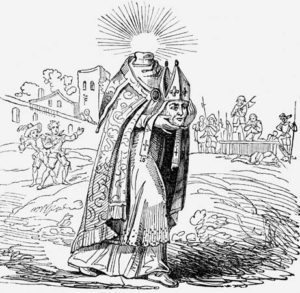
\includegraphics[scale=.5]{a20180830LosingOnesHead-img001.jpg} 
\caption{Saint Denys}
\end{wrapfigure}

\textbf{St Denis}, an early bishop of Paris, was martyred by decapitation at Montmartre. He then picked up his head, held it in front of his heart, and then walked several kilometres. The esoteric significance of this story is that the knowledge of the head needs to become subservient to the knowledge of the heart. \textbf{Rene Guenon} explains this distinction:

\begin{quotex}
Reason, which is only a mediate knowing faculty, is the strictly human mode of intelligence; intellectual intuition can be called supra-human, as it is a direct participation in universal intelligence which, residing in the heart, that is, at the being's very centre where lies his point of contact with the Divine, penetrates this being from within and illuminates him with its radiation. (\emph{The Symbolism of the Heart})

\end{quotex}
\paragraph{The New Dark Age}
\begin{quotex}
The time has long gone by when anyone who claims the title of philosopher can think of religion as a superfluity for the educated and an `opiate for the masses'. It is the only known explosive in the economy of that delicate internal-combustion engine, the human mind. Peoples rich in religious energy can overcome all obstacles and attain any height in the scale of civilization. Peoples that have reached the top of a hill by the wise use of religious energy may then decide to do without it; they can still move, but they can only move downhill, and when they come to the bottom of the hill they stop. \flright{\textsc{Robin Collingwood}}

\end{quotex}
Matter is darkness and consciousness is light. Yet our age considers materialism, the notion that nothing exists but matter, to be the sign of intelligence. \textbf{Sigmund Freud} showed us how there is a drive in his patients toward matter, which he called the death instinct. Collectively, our age loves death. It tries to blot out consciousness with drugs, noise, and distractions. That is considered to be the intelligent option.

Westerners today should be deliriously happy, as social goals like sexual liberation have been achieved. Yet reports of mental illness are high as well as both legal and illegal use of psychotropic drugs. If we are simply material beings, then there should be a material solution to the problems of life.

It is actually materialism that is the opiate of the masses. It absolves them from dealing with their faults in a serious way and from facing the consequences of their postmortem states.

We can see that the light eliminates darkness, yet no one can explain how darkness creates light.

\paragraph{Thinking}
Perhaps some examples of the three levels of knowledge discussed in the previous post will be helpful.

Most people, assuming they bother to think at all, are constrained to the level of opinion, or \emph{doxa}. They regard every discussion like a court case, with each side arguing for a predetermined outcome. Hence, such a person will accumulate facts and opinions that he feels will support his point of view, and his debating partner will do the same. These opinions are isolated from each other and don't become a coherent whole unless accidentally.

At a higher level, a person is able to reason effectively; that is \emph{dianoia}. He attempts to find the unifying factor by discovering the idea that accounts for the facts. That is the most likely story. However, its defect is that it is always subject to disproof or modification.

The ability to reason properly is actually quite difficult and most people overestimate their skill. Geometry is good practice, so Plato required a knowledge of geometry for his students. Advances in mathematics, such as statistical methods, game theory, and so on, have added more difficulties. In particular, statistical arguments are particularly difficult for most.

\emph{Episteme}, or intuition, is beyond argument. We can point to Euclid's axioms and postulates as examples. Either you understand them or you don't. You can't prove them or argue about them. The exception is the fifth postulate which has not been so obvious. It turns out, in fact, that alterations in that postulate lead to other, consistent geometries. Yet, the denial of the other axioms and postulates make geometry itself impossible.

The example Valentin Tomberg gave of such an intuition is the cosmos as an “ordered whole”. The scientist implicitly accepts this since he expects his experiments to lead to consistent results; moreover, the laws he discovers should be true across the universe.

The same is true for the religious person. God is the principle of being (the whole) and the Logos (order) is coextensive with God. Again, there is no empirical demonstration nor logical proof. One either understands it or not. It is not the same as a personal, subjective, or arbitrary conviction.

Unfortunately, in discussions of the higher things, people tend to move at the levels of doxa and dianoia indiscriminately. This makes communication impossible.

Yet the effort must be made. Meditation on certain ideas will help one reach the spiritual ideal. Then one can see.



\flrightit{Posted on 2018-08-30 by Cologero }
